\clearpage

\section{Opaque without Survivability - European Optical Network} \label{Realistic_Network}

In this case study we focus on the opaque case without survivability for the realistic network.

\subsection{Physical Network Topology}
\begin{tcolorbox}	
\begin{tabular}{p{2.75cm} p{0.2cm} p{10.5cm}} 	
\textbf{Student Name}  &:& Tiago Esteves    (October 03, 2017 - )\\
\end{tabular}
\end{tcolorbox}

The real network chosen for this work is the EON (European Optical Network).

\begin{figure}[h!]
\centering
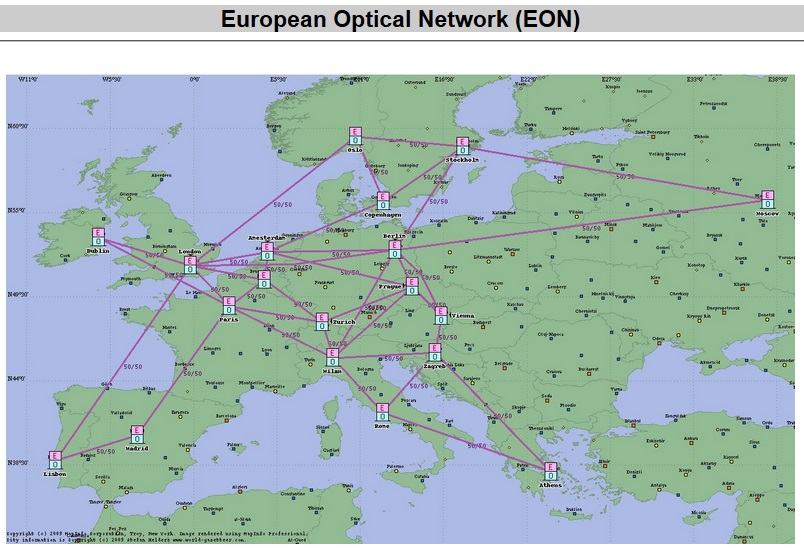
\includegraphics[width=\textwidth]{EON_Rede_Realista}
\caption{Physical topology of the realistic network.}
\end{figure}

In this real case we have take into consideration the table \ref{table_real_net} because it is through it that we can see the values of the variables associated with this network.

\begin{table}[h!]
\centering
\begin{tabular}{|| c | c | c||}
 \hline
 Constant & Description & Value \\
 \hline\hline
 N & Number of nodes & 19 \\
 L & Number of bidirectional links & 37 \\
 <$\delta$> & Node out-degree & 3.89 \\
 <len> & Mean link length (km) & 753.76 \\
 <h> & Mean number of hops for working paths & 2.3 \\
 <h'> & Mean number of hops for backup paths & 3.2 \\
 \hline
\end{tabular}
\caption{Table of realistic network values}
\label{table_real_net}
\end{table}

\newpage
Through the previous figure we can see how nodes are organized geographically and the distance matrix created on the next page is constructed based on real distances between them.
For a better understanding of the distances matrix the table \ref{city_nodes_realnet} was created to assign to each city a number of a node in the network.


\begin{table}[h!]
\centering
\begin{tabular}{|| c | c ||}
 \hline
 City & Node \\
 \hline\hline
 Oslo & 1 \\
 Stockholm & 2 \\
 Moscow & 3 \\
 Copenhagen & 4 \\
 Berlin & 5 \\
 Prague & 6 \\
 Vienna & 7 \\
 Zagreb & 8 \\
 Athens & 9 \\
 Rome & 10 \\
 Milan & 11 \\
 Zurich & 12 \\
 Brussels & 13 \\
 Amesterdan & 14 \\
 London & 15 \\
 Dublin & 16 \\
 Paris & 17 \\
 Madrid & 18 \\
 Lisbon & 19 \\
 \hline
\end{tabular}
\caption{Table of city and respective node}
\label{city_nodes_realnet}
\end{table}


The values indicated in the distance matrix, referred to below, are expressed in kilometers (Km).
For this network we must also create matrices of ODU's to determine the total traffic used in each scenario but in this case only the matrices for low traffic are elucidated.

\begin{sidewaysfigure}

\[
Dist=
  \begin{pmatrix}
    0 & 417 & 0 & 484 & 0 & 0 & 0 & 0 & 0 & 0 & 0 & 0 & 0 & 0 & 1155 & 0 & 0 & 0 & 0 \\
    417 & 0 & 1228 & 523 & 811 & 0 & 0 & 0 & 0 & 0 & 0 & 0 & 0 & 0 & 0 & 0 & 0 & 0 & 0 \\
    0 & 1228 & 0 & 0 & 1611 & 0 & 0 & 0 & 0 & 0 & 0 & 0 & 0 & 0 & 0 & 0 & 0 & 0 & 0 \\
    484 & 523 & 0 & 0 & 0 & 0 & 0 & 0 & 0 & 0 & 0 & 0 & 0 & 622 & 0 & 0 & 0 & 0 & 0 \\
    0 & 811 & 1611 & 0 & 0 & 281 & 524 & 0 & 0 & 0 & 843 & 0 & 0 & 577 & 933 & 0 & 0 & 0 & 0 \\
    0 & 0 & 0 & 0 & 281 & 0 & 251 & 0 & 0 & 0 & 646 & 527 & 0 & 712 & 0 & 0 & 0 & 0 & 0 \\
    0 & 0 & 0 & 0 & 524 & 251 & 0 & 268 & 0 & 0 & 0 & 0 & 0 & 0 & 0 & 0 & 0 & 0 & 0 \\
    0 & 0 & 0 & 0 & 0 & 0 & 268 & 0 & 1081 & 518 & 530 & 0 & 0 & 0 & 0 & 0 & 0 & 0 & 0 \\
    0 & 0 & 0 & 0 & 0 & 0 & 0 & 1081 & 0 & 1052 & 0 & 0 & 0 & 0 & 0 & 0 & 0 & 0 & 0 \\
    0 & 0 & 0 & 0 & 0 & 0 & 0 & 518 & 1052 & 0 & 477 & 0 & 0 & 0 & 0 & 0 & 0 & 0 & 0 \\
    0 & 0 & 0 & 0 & 843 & 646 & 0 & 530 & 0 & 477 & 0 & 219 & 0 & 0 & 0 & 0 & 640 & 0 & 0 \\
    0 & 0 & 0 & 0 & 0 & 646 & 0 & 0 & 0 & 0 & 219 & 0 & 493 & 0 & 0 & 0 & 488 & 0 & 0 \\
    0 & 0 & 0 & 0 & 0 & 0 & 0 & 0 & 0 & 0 & 0 & 493 & 0 & 173 & 321 & 0 & 264 & 0 & 0 \\
    0 & 0 & 0 & 622 & 577 & 712 & 0 & 0 & 0 & 0 & 0 & 0 & 173 & 0 & 358 & 0 & 0 & 0 & 0 \\
    1155 & 0 & 0 & 0 & 933 & 0 & 0 & 0 & 0 & 0 & 0 & 0 & 321 & 358 & 0 & 464 & 344 & 0 & 1587 \\
    0 & 0 & 0 & 0 & 0 & 0 & 0 & 0 & 0 & 0 & 0 & 0 & 0 & 0 & 464 & 0 & 782 & 0 & 0 \\
    0 & 0 & 0 & 0 & 0 & 0 & 0 & 0 & 0 & 0 & 640 & 488 & 264 & 0 & 344 & 782 & 0 & 1054 & 0 \\
    0 & 0 & 0 & 0 & 0 & 0 & 0 & 0 & 0 & 0 & 0 & 0 & 0 & 0 & 0 & 0 & 1054 & 0 & 503 \\
    0 & 0 & 0 & 0 & 0 & 0 & 0 & 0 & 0 & 0 & 0 & 0 & 0 & 0 & 1587 & 0 & 0 & 503 & 0
  \end{pmatrix}
\]
\end{sidewaysfigure}

\[
ODU0=
  \begin{bmatrix}
    0 & 1 & 1 & 1 & 1 & 1 & 1 & 1 & 1 & 1 & 1 & 1 & 1 & 1 & 1 & 1 & 1 & 1 & 1 \\
    1 & 0 & 1 & 1 & 1 & 1 & 1 & 1 & 1 & 1 & 1 & 1 & 1 & 1 & 1 & 1 & 1 & 1 & 1 \\
    1 & 1 & 0 & 1 & 1 & 1 & 1 & 1 & 1 & 1 & 1 & 1 & 1 & 1 & 1 & 1 & 1 & 1 & 1 \\
    1 & 1 & 1 & 0 & 1 & 1 & 1 & 1 & 1 & 1 & 1 & 1 & 1 & 1 & 1 & 1 & 1 & 1 & 1 \\
    1 & 1 & 1 & 1 & 0 & 1 & 1 & 1 & 1 & 1 & 1 & 1 & 1 & 1 & 1 & 1 & 1 & 1 & 1 \\
    1 & 1 & 1 & 1 & 1 & 0 & 1 & 1 & 1 & 1 & 1 & 1 & 1 & 1 & 1 & 1 & 1 & 1 & 1 \\
    1 & 1 & 1 & 1 & 1 & 1 & 0 & 1 & 1 & 1 & 1 & 1 & 1 & 1 & 1 & 1 & 1 & 1 & 1 \\
    1 & 1 & 1 & 1 & 1 & 1 & 1 & 0 & 1 & 1 & 1 & 1 & 1 & 1 & 1 & 1 & 1 & 1 & 1 \\
    1 & 1 & 1 & 1 & 1 & 1 & 1 & 1 & 0 & 1 & 1 & 1 & 1 & 0 & 0 & 0 & 0 & 0 & 0 \\
    1 & 1 & 1 & 1 & 1 & 1 & 1 & 1 & 1 & 0 & 0 & 0 & 0 & 0 & 0 & 0 & 0 & 0 & 0 \\
    1 & 1 & 1 & 1 & 1 & 1 & 1 & 1 & 1 & 0 & 0 & 0 & 0 & 0 & 0 & 0 & 0 & 0 & 0 \\
    1 & 1 & 1 & 1 & 1 & 1 & 1 & 1 & 1 & 0 & 0 & 0 & 0 & 0 & 0 & 0 & 0 & 0 & 0 \\
    1 & 1 & 1 & 1 & 1 & 1 & 1 & 1 & 1 & 0 & 0 & 0 & 0 & 0 & 0 & 0 & 0 & 0 & 0 \\
    1 & 1 & 1 & 1 & 1 & 1 & 1 & 1 & 0 & 0 & 0 & 0 & 0 & 0 & 0 & 0 & 0 & 0 & 0 \\
    1 & 1 & 1 & 1 & 1 & 1 & 1 & 1 & 0 & 0 & 0 & 0 & 0 & 0 & 0 & 0 & 0 & 0 & 0 \\
    1 & 1 & 1 & 1 & 1 & 1 & 1 & 1 & 0 & 0 & 0 & 0 & 0 & 0 & 0 & 0 & 0 & 0 & 0 \\
    1 & 1 & 1 & 1 & 1 & 1 & 1 & 1 & 0 & 0 & 0 & 0 & 0 & 0 & 0 & 0 & 0 & 0 & 0 \\
    1 & 1 & 1 & 1 & 1 & 1 & 1 & 1 & 0 & 0 & 0 & 0 & 0 & 0 & 0 & 0 & 0 & 0 & 0 \\
    1 & 1 & 1 & 1 & 1 & 1 & 1 & 1 & 0 & 0 & 0 & 0 & 0 & 0 & 0 & 0 & 0 & 0 & 0
  \end{bmatrix}
\]

\vspace{15pt}

\[
ODU1=
  \begin{bmatrix}
    0 & 1 & 0 & 0 & 0 & 0 & 0 & 0 & 0 & 0 & 1 & 1 & 1 & 1 & 1 & 1 & 1 & 0 & 0 \\
    1 & 0 & 0 & 0 & 0 & 0 & 0 & 0 & 0 & 0 & 1 & 1 & 1 & 1 & 1 & 1 & 1 & 1 & 1 \\
    0 & 0 & 0 & 0 & 0 & 1 & 1 & 1 & 1 & 1 & 1 & 1 & 1 & 1 & 1 & 1 & 1 & 1 & 1 \\
    0 & 0 & 0 & 0 & 1 & 1 & 1 & 1 & 1 & 1 & 1 & 1 & 1 & 1 & 1 & 1 & 1 & 1 & 1 \\
    0 & 0 & 0 & 1 & 0 & 1 & 1 & 1 & 1 & 1 & 1 & 1 & 1 & 1 & 1 & 1 & 1 & 1 & 1 \\
    0 & 0 & 1 & 1 & 1 & 0 & 1 & 1 & 1 & 1 & 1 & 1 & 1 & 1 & 1 & 1 & 1 & 1 & 1 \\
    0 & 0 & 1 & 1 & 1 & 1 & 0 & 1 & 1 & 1 & 1 & 1 & 1 & 1 & 1 & 1 & 1 & 1 & 1 \\
    0 & 0 & 1 & 1 & 1 & 1 & 1 & 0 & 1 & 1 & 1 & 1 & 1 & 1 & 1 & 1 & 1 & 1 & 1 \\
    0 & 0 & 1 & 1 & 1 & 1 & 1 & 1 & 0 & 1 & 1 & 1 & 1 & 0 & 0 & 0 & 0 & 0 & 0 \\
    0 & 0 & 1 & 1 & 1 & 1 & 1 & 1 & 1 & 0 & 0 & 0 & 0 & 0 & 0 & 0 & 0 & 0 & 0 \\
    1 & 1 & 1 & 1 & 1 & 1 & 1 & 1 & 1 & 0 & 0 & 0 & 0 & 0 & 0 & 0 & 0 & 0 & 0 \\
    1 & 1 & 1 & 1 & 1 & 1 & 1 & 1 & 1 & 0 & 0 & 0 & 0 & 0 & 0 & 0 & 0 & 0 & 0 \\
    1 & 1 & 1 & 1 & 1 & 1 & 1 & 1 & 1 & 0 & 0 & 0 & 0 & 0 & 0 & 0 & 0 & 0 & 0 \\
    1 & 1 & 1 & 1 & 1 & 1 & 1 & 1 & 0 & 0 & 0 & 0 & 0 & 0 & 0 & 0 & 0 & 0 & 0 \\
    1 & 1 & 1 & 1 & 1 & 1 & 1 & 1 & 0 & 0 & 0 & 0 & 0 & 0 & 0 & 0 & 0 & 0 & 0 \\
    1 & 1 & 1 & 1 & 1 & 1 & 1 & 1 & 0 & 0 & 0 & 0 & 0 & 0 & 0 & 0 & 0 & 0 & 0 \\
    1 & 1 & 1 & 1 & 1 & 1 & 1 & 1 & 0 & 0 & 0 & 0 & 0 & 0 & 0 & 0 & 0 & 0 & 0 \\
    0 & 1 & 1 & 1 & 1 & 1 & 1 & 1 & 0 & 0 & 0 & 0 & 0 & 0 & 0 & 0 & 0 & 0 & 0 \\
    0 & 1 & 1 & 1 & 1 & 1 & 1 & 1 & 0 & 0 & 0 & 0 & 0 & 0 & 0 & 0 & 0 & 0 & 0
  \end{bmatrix}
\]


\[
ODU2=
  \begin{bmatrix}
    0 & 1 & 1 & 2 & 2 & 0 & 0 & 0 & 0 & 0 & 0 & 0 & 0 & 0 & 0 & 0 & 0 & 0 & 0 \\
    1 & 0 & 2 & 2 & 2 & 2 & 0 & 0 & 0 & 0 & 0 & 0 & 0 & 0 & 0 & 0 & 0 & 0 & 0 \\
    1 & 2 & 0 & 2 & 2 & 2 & 0 & 0 & 0 & 0 & 0 & 0 & 0 & 0 & 0 & 0 & 0 & 0 & 0 \\
    2 & 2 & 2 & 0 & 2 & 2 & 2 & 0 & 0 & 0 & 0 & 0 & 0 & 0 & 0 & 0 & 0 & 0 & 0 \\
    2 & 2 & 2 & 2 & 0 & 0 & 0 & 0 & 0 & 0 & 0 & 0 & 0 & 0 & 0 & 0 & 0 & 0 & 0 \\
    0 & 2 & 2 & 2 & 0 & 0 & 2 & 0 & 2 & 2 & 0 & 0 & 0 & 0 & 0 & 0 & 0 & 0 & 0 \\
    0 & 0 & 0 & 2 & 0 & 2 & 0 & 0 & 0 & 0 & 0 & 0 & 0 & 0 & 0 & 0 & 0 & 0 & 0 \\
    0 & 0 & 0 & 0 & 0 & 0 & 0 & 0 & 0 & 0 & 0 & 0 & 0 & 0 & 0 & 0 & 0 & 0 & 0 \\
    0 & 0 & 0 & 0 & 0 & 2 & 0 & 0 & 0 & 0 & 0 & 0 & 0 & 0 & 0 & 0 & 0 & 0 & 0 \\
    0 & 0 & 0 & 0 & 0 & 2 & 0 & 0 & 0 & 0 & 0 & 0 & 0 & 0 & 0 & 0 & 0 & 0 & 0 \\
    0 & 0 & 0 & 0 & 0 & 0 & 0 & 0 & 0 & 0 & 0 & 0 & 0 & 0 & 0 & 0 & 0 & 0 & 0 \\
    0 & 0 & 0 & 0 & 0 & 0 & 0 & 0 & 0 & 0 & 0 & 0 & 0 & 0 & 0 & 0 & 0 & 0 & 0 \\
    0 & 0 & 0 & 0 & 0 & 0 & 0 & 0 & 0 & 0 & 0 & 0 & 0 & 0 & 0 & 0 & 0 & 0 & 0 \\
    0 & 0 & 0 & 0 & 0 & 0 & 0 & 0 & 0 & 0 & 0 & 0 & 0 & 0 & 0 & 0 & 0 & 0 & 0 \\
    0 & 0 & 0 & 0 & 0 & 0 & 0 & 0 & 0 & 0 & 0 & 0 & 0 & 0 & 0 & 0 & 0 & 0 & 0 \\
    0 & 0 & 0 & 0 & 0 & 0 & 0 & 0 & 0 & 0 & 0 & 0 & 0 & 0 & 0 & 0 & 0 & 0 & 0 \\
    0 & 0 & 0 & 0 & 0 & 0 & 0 & 0 & 0 & 0 & 0 & 0 & 0 & 0 & 0 & 0 & 0 & 0 & 0 \\
    0 & 0 & 0 & 0 & 0 & 0 & 0 & 0 & 0 & 0 & 0 & 0 & 0 & 0 & 0 & 0 & 0 & 0 & 0 \\
    0 & 0 & 0 & 0 & 0 & 0 & 0 & 0 & 0 & 0 & 0 & 0 & 0 & 0 & 0 & 0 & 0 & 0 & 0
  \end{bmatrix}
\]

\vspace{15pt}

\[
ODU3=
  \begin{bmatrix}
    0 & 0 & 0 & 0 & 0 & 0 & 0 & 0 & 0 & 0 & 0 & 0 & 0 & 0 & 0 & 0 & 0 & 0 & 0 \\
    0 & 0 & 0 & 0 & 0 & 0 & 0 & 0 & 0 & 0 & 0 & 0 & 0 & 0 & 0 & 0 & 0 & 0 & 0 \\
    0 & 0 & 0 & 0 & 0 & 0 & 0 & 0 & 0 & 0 & 0 & 0 & 0 & 0 & 0 & 0 & 0 & 0 & 0 \\
    0 & 0 & 0 & 0 & 0 & 0 & 0 & 0 & 0 & 0 & 0 & 0 & 0 & 0 & 0 & 0 & 0 & 0 & 0 \\
    0 & 0 & 0 & 0 & 0 & 0 & 0 & 0 & 0 & 0 & 0 & 0 & 0 & 0 & 0 & 0 & 0 & 0 & 0 \\
    0 & 0 & 0 & 0 & 0 & 0 & 0 & 0 & 0 & 0 & 0 & 0 & 0 & 0 & 0 & 0 & 0 & 0 & 0 \\
    0 & 0 & 0 & 0 & 0 & 0 & 0 & 0 & 0 & 0 & 0 & 0 & 0 & 0 & 0 & 0 & 0 & 0 & 1 \\
    0 & 0 & 0 & 0 & 0 & 0 & 0 & 0 & 0 & 0 & 0 & 0 & 0 & 0 & 0 & 0 & 0 & 0 & 1 \\
    0 & 0 & 0 & 0 & 0 & 0 & 0 & 0 & 0 & 0 & 0 & 0 & 0 & 0 & 0 & 0 & 0 & 0 & 1 \\
    0 & 0 & 0 & 0 & 0 & 0 & 0 & 0 & 0 & 0 & 0 & 0 & 0 & 0 & 0 & 0 & 0 & 0 & 1 \\
    0 & 0 & 0 & 0 & 0 & 0 & 0 & 0 & 0 & 0 & 0 & 0 & 0 & 0 & 0 & 0 & 0 & 0 & 1 \\
    0 & 0 & 0 & 0 & 0 & 0 & 0 & 0 & 0 & 0 & 0 & 0 & 0 & 0 & 0 & 0 & 0 & 0 & 1 \\
    0 & 0 & 0 & 0 & 0 & 0 & 0 & 0 & 0 & 0 & 0 & 0 & 0 & 0 & 0 & 0 & 0 & 0 & 1 \\
    0 & 0 & 0 & 0 & 0 & 0 & 0 & 0 & 0 & 0 & 0 & 0 & 0 & 0 & 0 & 0 & 0 & 0 & 1 \\
    0 & 0 & 0 & 0 & 0 & 0 & 0 & 0 & 0 & 0 & 0 & 0 & 0 & 0 & 0 & 0 & 0 & 0 & 1 \\
    0 & 0 & 0 & 0 & 0 & 0 & 0 & 0 & 0 & 0 & 0 & 0 & 0 & 0 & 0 & 0 & 0 & 0 & 1 \\
    0 & 0 & 0 & 0 & 0 & 0 & 0 & 0 & 0 & 0 & 0 & 0 & 0 & 0 & 0 & 0 & 0 & 0 & 1 \\
    0 & 0 & 0 & 0 & 0 & 0 & 0 & 0 & 0 & 0 & 0 & 0 & 0 & 0 & 0 & 0 & 0 & 0 & 1 \\
    0 & 0 & 0 & 0 & 0 & 0 & 1 & 1 & 1 & 1 & 1 & 1 & 1 & 1 & 1 & 1 & 1 & 1 & 0
  \end{bmatrix}
\]


\[
ODU4=
  \begin{bmatrix}
    0 & 1 & 0 & 0 & 0 & 0 & 0 & 0 & 0 & 0 & 0 & 0 & 0 & 0 & 0 & 0 & 0 & 0 & 0 \\
    1 & 0 & 0 & 0 & 0 & 0 & 0 & 0 & 0 & 0 & 0 & 0 & 0 & 0 & 0 & 0 & 0 & 0 & 0 \\
    0 & 0 & 0 & 1 & 0 & 0 & 0 & 0 & 0 & 0 & 0 & 0 & 0 & 0 & 0 & 0 & 0 & 0 & 0 \\
    0 & 0 & 1 & 0 & 0 & 0 & 0 & 0 & 0 & 0 & 0 & 0 & 0 & 0 & 0 & 0 & 0 & 0 & 0 \\
    0 & 0 & 0 & 0 & 0 & 0 & 0 & 1 & 0 & 0 & 0 & 0 & 0 & 0 & 0 & 0 & 0 & 0 & 0 \\
    0 & 0 & 0 & 0 & 0 & 0 & 1 & 0 & 0 & 0 & 0 & 0 & 0 & 0 & 0 & 0 & 0 & 0 & 0 \\
    0 & 0 & 0 & 0 & 0 & 1 & 0 & 0 & 0 & 0 & 0 & 0 & 0 & 0 & 0 & 0 & 0 & 0 & 0 \\
    0 & 0 & 0 & 0 & 1 & 0 & 0 & 0 & 0 & 0 & 0 & 0 & 0 & 0 & 0 & 0 & 0 & 0 & 0 \\
    0 & 0 & 0 & 0 & 0 & 0 & 0 & 0 & 0 & 1 & 0 & 0 & 0 & 0 & 0 & 0 & 0 & 0 & 0 \\
    0 & 0 & 0 & 0 & 0 & 0 & 0 & 0 & 1 & 0 & 0 & 0 & 0 & 0 & 0 & 0 & 0 & 0 & 0 \\
    0 & 0 & 0 & 0 & 0 & 0 & 0 & 0 & 0 & 0 & 0 & 0 & 0 & 0 & 0 & 0 & 0 & 0 & 0 \\
    0 & 0 & 0 & 0 & 0 & 0 & 0 & 0 & 0 & 0 & 0 & 0 & 1 & 0 & 0 & 0 & 0 & 0 & 0 \\
    0 & 0 & 0 & 0 & 0 & 0 & 0 & 0 & 0 & 0 & 0 & 1 & 0 & 0 & 0 & 0 & 0 & 0 & 0 \\
    0 & 0 & 0 & 0 & 0 & 0 & 0 & 0 & 0 & 0 & 0 & 0 & 0 & 0 & 0 & 0 & 0 & 0 & 0 \\
    0 & 0 & 0 & 0 & 0 & 0 & 0 & 0 & 0 & 0 & 0 & 0 & 0 & 0 & 0 & 1 & 0 & 0 & 0 \\
    0 & 0 & 0 & 0 & 0 & 0 & 0 & 0 & 0 & 0 & 0 & 0 & 0 & 0 & 1 & 0 & 0 & 0 & 0 \\
    0 & 0 & 0 & 0 & 0 & 0 & 0 & 0 & 0 & 0 & 0 & 0 & 0 & 0 & 0 & 0 & 0 & 0 & 0 \\
    0 & 0 & 0 & 0 & 0 & 0 & 0 & 0 & 0 & 0 & 0 & 0 & 0 & 0 & 0 & 0 & 0 & 0 & 1 \\
    0 & 0 & 0 & 0 & 0 & 0 & 0 & 0 & 0 & 0 & 0 & 0 & 0 & 0 & 0 & 0 & 0 & 1 & 0
  \end{bmatrix}
\]

\vspace{11pt}
In the traffic matrices each ODU, referred previously, has its respective value being that the ODU0 corresponds to 1.25 Gbits/s, ODU1 to 2.5 Gbits/s, ODU2 to 10 Gbits/s, ODU3 to 40 Gbits/s and finally the ODU4 corresponds to 100 Gbits/s.
As we can see these matrices are bidirectional because they are symmetric matrices and as such the traffic sent in one direction must be the same traffic sent in the opposite direction.

Through these ODU's we can calculate total network traffic for the low traffic scenario:\\

$T_1^0$ = 240x1.25 = 300 Gbits/s \qquad
$T_1^1$ = 200x2.5 = 500 Gbits/s \qquad
$T_1^2$ = 64x10 = 640 Gbits/s \\

$T_1^3$ = 24x40 = 960 Gbits/s \quad
$T_1^4$ = 16x100 = 1600 Gbits/s \\

$T_{1}$ = 300 + 500 + 640 + 960 + 1600 = 4000 Gbits/s \qquad
$T$ = 4000/2 = 2 Tbits/s\\

Where the variable $T_1^x$ represents the unidirectional traffic of the ODUx, for example, $T_1^3$ represents the unidirectional traffic of the ODU3 and $T_1^4$ represents the unidirectional traffic of the ODU4. The variable $T_{1}$ represents the total of unidirectional traffic that is injected into the network and finally the variable $T$ represents the total of bidirectional traffic.\\

Again, we can thus conclude that the total traffic for the two scenarios is as follows:
\begin{itemize}
  \item Low Traffic: \textbf{2 TBits/s}
  \item High Traffic: \textbf{20 TBits/s}
\end{itemize}


\subsection{Dimensioning using Analytical Model}
\begin{tcolorbox}	
\begin{tabular}{p{2.75cm} p{0.2cm} p{10.5cm}} 	
\textbf{Student Name}  &:& Tiago Esteves    (October 03, 2017 - )\\
\end{tabular}
\end{tcolorbox}

In this section we will do the dimensioning of the network mentioned in the previous subsection to calculate the value of your CAPEX, for this we will use the analytical formulations so as to obtain the best solution but for this we will also have to take into account the cost of the equipment used that can be consulted in table \ref{table_cost_opaque}.
The formulas and calculations needed for the CAPEX of the network are the same as in the previous case (reference network) and therefore only the results obtained will be presented.\\

As described in the subsection of the network topology we have two values of network traffic, low traffic and high traffic, soon we will get two different CAPEX. Finally we have to take into account that as it is the opaque transport mode, the value of $\xi$ is 1 and because it is without survivability, the value of $<k>$ is 0. Then we can rewrite the equations.\\

\textbf{Scenario 1: Realistic Network Low Traffic}\\

Using equation \ref{demands}:\\

$D$ = $\frac{1}{2}$ * $($ 1 + 1 $)$ * $($ $\frac{4000}{100}$ $)$ \qquad \qquad $D$ = 40\\

Replacing in equation \ref{optical_channels}:\\

$<w>$ = $($ $\frac{40 * 2.3}{37}$ $)$ * $($ 1 + 0$)$ \qquad \qquad $<w>$ = 3\\

Using equation \ref{amplifiers}:\\

$N^R$ $\backsimeq$ L * $<N^R>$ \\

$<N^R>$ = $\frac{<len>}{span}-1$\\

$<N^R>$ = $\frac{<753.76>}{100}-1$\\

$N^R$ = 259\\

Finally, replacing all in equation \ref{analytical_linkCosts} the Link Cost is:\\

$C_L$ = $($2 * 37 * 15000$)$ + $($2 * 37 * 5000 * 100 * 3$)$ + $($259 * 4000$)$\\

$C_L$ = \textbf{113 146 000 \euro}\\

In relation to the cost of the nodes we first use the equation \ref{average_demand}:\\

$<d>$ = $\frac{2 * 40}{19}$ \qquad \qquad $<d>$ = 4.21\\

Replacing in equation \ref{Pexc_opaque}:\\

$P_{exc}$ = 4.21 * $[$1 + $($1 + $0$ $)$ * 2.3$]$ \qquad \quad $P_{exc}$ = 13.893 \\

Finally, replacing all in equation \ref{analytical_electricalCost} the Node Cost is:\\

$C_N$ = $C_{exc}$ = 19 * $($10000 + $($1000 * 100 * 13.893 $)$ $)$\\

$C_N$ = \textbf{26 589 700 \euro}\\

The CAPEX is:\\
$CAPEX$ = 113 146 000 + 26 589 700\\

$CAPEX$ = \textbf{139 732 700 \euro}\\

\textbf{Scenario 2: Reference Network High Traffic}\\

Using equation \ref{demands}:\\

$D$ = $\frac{1}{2}$ * $($ 1 + 1 $)$ * $($ $\frac{40000}{100}$ $)$ \qquad \qquad $D$ = 400\\

replacing in equation \ref{optical_channels}:\\

$<w>$ = $($ $\frac{400 * 2.3}{37}$ $)$ * $($ 1 + 0$)$ \qquad \quad $<w>$ = 25\\

Finally, replacing all in equation \ref{analytical_linkCosts} the Link Cost is:\\

$C_L$ = $($2 * 37 * 15000$)$ + $($2 * 37 * 5000 * 100 * 25$)$ + $($259 * 4000$)$\\

$C_L$ = \textbf{927 146 000 \euro}\\

In relation to the cost of the nodes we first use the equation \ref{average_demand}:\\

$<d>$ = $\frac{2 * 400}{19}$ \qquad \qquad $<d>$ = 42.105\\

Replacing in equation \ref{Pexc_opaque}:\\

$P_{exc}$ = 42.105 * $[$1 + $($1 + $0$ $)$ * 2.3$]$ \qquad \qquad $P_{exc}$ = 138.9465 \\

Finally, replacing all in equation \ref{analytical_electricalCost} the Node Cost is:\\

$C_N$ = $C_{exc}$ = 19 * $($10000 + $($1000 * 100 * 138.9465 $)$ $)$\\

$C_N$ = \textbf{246 188 350 \euro}\\

The CAPEX is:\\
$CAPEX$ = 927 146 000 + 246 188 350\\

$CAPEX$ = \textbf{1 191 334 350 \euro}\\


\subsection{Dimensioning using ILP}
\begin{tcolorbox}	
\begin{tabular}{p{2.75cm} p{0.2cm} p{10.5cm}} 	
\textbf{Student Name}  &:& Tiago Esteves    (October 03, 2017 - )\\
\end{tabular}
\end{tcolorbox}

In this section we will do the dimensioning of the network mentioned in the previous section to calculate the value of your CAPEX.
The initial subsection is the same as the subsection of the previous case so in this case it will be omitted presenting only the subsection of the results.\\

\textbf{Scenario 1: Realistic Network Low Traffic} \label{Scenario3_opaque} \\

This real network consists of many nodes and with many links between them as such the lpsolve takes immense time to get an optimal solution. Therefore, in this two cases, the execution time was defined as being two days (48 hours) and after that time presented the best solution. In this scenario we used the table \ref{table_real_net} and in the table \ref{result_ILP3_without} we can see the values calculated through MatLab and using the values indicated in table \ref{table_cost_opaque} we can finally calculate the CAPEX value.\\

Using equation \ref{linkCosts} : \\
$C_L$ = $($2 * 15 000 * 37$)$ + $($2 * 5 000 * 100 *  $)$ + $($ * 4 000$)$ \\
$C_L$ = \textbf{\euro} \\

Using equation \ref{electricalCostOpaque} : \\
$C_{exc}$ = $($19 * 10 000$)$ + 1 000 * $($4 000 + $($2 *  * 100$)$ $)$ \\
$C_N$ = $C_{exc}$ = \textbf{ \euro} \\

$CAPEX$ =  +  = \textbf{ \euro}\\

\begin{table}[h!]
\centering
\begin{tabular}{|| c | c||}
 \hline
 Number of optical channels & Value \\
 \hline\hline
in link (1,2) &  \\
in link (1,4) &  \\
in link (1,15) &  \\
in link (2,3) &  \\
in link (2,4) &  \\
in link (2,5) &  \\
in link (3,5) &  \\
in link (4,14) &  \\
in link (5,6) &  \\
in link (5,7) &  \\
in link (5,11) &  \\
in link (5,14) &  \\
in link (5,15) &  \\
in link (6,7) &  \\
in link (6,11) &  \\
in link (6,12) &  \\
in link (6,14) &  \\
in link (7,8) &  \\
in link (8,9) &  \\
in link (8,10) &  \\
in link (8,11) &  \\
in link (9,10) &  \\
in link (10,11) &  \\
in link (11,12) &  \\
in link (11,17) &  \\
in link (12,13) &  \\
in link (12,17) &  \\
in link (13,14) &  \\
in link (13,15) &  \\
in link (13,17) &  \\
in link (14,15) &  \\
in link (15,16) &  \\
in link (15,17) &  \\
in link (15,19) &  \\
in link (16,17) &  \\
in link (17,18) &  \\
in link (18,19) &  \\
\hline
\end{tabular}
\caption{Table with results}
\label{result_ILP3_without}
\end{table}

\textbf{Scenario 2: Realistic Network High Traffic} \label{Scenario4_opaque} \\
In this scenario we used again the table \ref{table_real_net} and in the table \ref{result_ILP4_without} we can see the values calculated through MatLab and using the values indicated in table \ref{table_cost_opaque} we can finally calculate the CAPEX value. \\

\begin{table}[h!]
\centering
\begin{tabular}{|| c | c||}
 \hline
 Number of optical channels & Value \\
 \hline\hline
 in link (1,2) &  \\
in link (1,4) &  \\
in link (1,15) &  \\
in link (2,3) &  \\
in link (2,4) &  \\
in link (2,5) &  \\
in link (3,5) &  \\
in link (4,14) &  \\
in link (5,6) &  \\
in link (5,7) &  \\
in link (5,11) &  \\
in link (5,14) &  \\
in link (5,15) &  \\
in link (6,7) &  \\
in link (6,11) &  \\
in link (6,12) &  \\
in link (6,14) &  \\
in link (7,8) &  \\
in link (8,9) &  \\
in link (8,10) &  \\
in link (8,11) &  \\
in link (9,10) &  \\
in link (10,11) &  \\
in link (11,12) &  \\
in link (11,17) &  \\
in link (12,13) &  \\
in link (12,17) &  \\
in link (13,14) &  \\
in link (13,15) &  \\
in link (13,17) &  \\
in link (14,15) &  \\
in link (15,16) &  \\
in link (15,17) &  \\
in link (15,19) &  \\
in link (16,17) &  \\
in link (17,18) &  \\
in link (18,19) &  \\
\hline
\end{tabular}
\caption{Table with results}
\label{result_ILP4_without}
\end{table}

Using equation \ref{linkCosts} : \\
$C_L$ = $($2 * 15 000 * 37$)$ + $($2 * 5 000 * 100 * $)$ + $($24 * 4 000$)$ \\
$C_L$ = \textbf{ \euro} \\

Using equation \ref{electricalCostOpaque} : \\
$C_{exc}$ = $($19 * 10 000$)$ + 1 000 * $($40 000 + $($2 * 100 * $)$ $)$ \\
$C_N$ = $C_{exc}$ = \textbf{ \euro} \\

$CAPEX$ =  +  = \textbf{ \euro}\\

\subsection{Dimensioning using Heuristics}

\subsubsection{Heuristics Results}

\subsection{Comparative Analysis}
